%
% Szakdolgozatminta az Eszterházy Károly Katolikus Egyetem
% matematika illetve informatika szakos hallgatóinak.
%

\documentclass[
% opciók nélkül: egyoldalas nyomtatás, elektronikus verzió
% twoside,     % kétoldalas nyomtatás
% tocnopagenum,% oldalszámozás a tartalomjegyzék után kezdődik
]{thesis-ekf}
\usepackage[T1]{fontenc}
\usepackage{hulipsum}
\PassOptionsToPackage{defaults=hu-min}{magyar.ldf}
\usepackage[magyar]{babel}
\usepackage{mathtools,amssymb,amsthm,pdfpages}
\footnotestyle{rule=fourth}

\newtheorem{tetel}{Tétel}[chapter]
\theoremstyle{definition}
\newtheorem{definicio}[tetel]{Definíció}
\theoremstyle{remark}
\newtheorem{megjegyzes}[tetel]{Megjegyzés}

\begin{document}
\institute{Matematikai és Informatikai Intézet}
\title{Programozható elektronikák alkalmazásai}
\author{Bagoly Gábor\\programtervező informatikus}
\supervisor{Dr. Geda Gábor\\egyetemi docens}
\city{Eger}
\date{2022}
\maketitle
\tableofcontents

\chapter*{Bevezetés}
\addcontentsline{toc}{chapter}{Bevezetés}
\hulipsum[1]
\cite{Fazekas}

\chapter{Fejezet címe}
\section{Szakasz címe}
\subsection{Alszakasz címe}
\hulipsum[1]
\cite[102.~oldal]{Fazekas}

\hulipsum[1]
\cite{Fazekas,Tomacs}

\begin{tetel}
Tétel szövege.
\end{tetel}

\begin{proof}
Bizonyítás szövege.
\end{proof}

\begin{definicio}
Definíció szövege.
\end{definicio}

\begin{megjegyzes}
Megjegyzés szövege.
\end{megjegyzes}

\chapter*{Összegzés}
\addcontentsline{toc}{chapter}{Összegzés}
\hulipsum[1]

\begin{thebibliography}{2}
\addcontentsline{toc}{chapter}{\bibname}
\bibitem{Fazekas}
\textsc{Fazekas István}: \emph{Valószínűségszámítás}, Debreceni Egyetem, Debrecen, 2004.
\bibitem{Tomacs}
\textsc{Tómács Tibor}: \emph{A valószínűségszámítás alapjai}, Líceum Kiadó, Eger, 2005.
\end{thebibliography}

% Aláírt, szkennelt nyilatkozat beillesztése a szakdolgozat végére
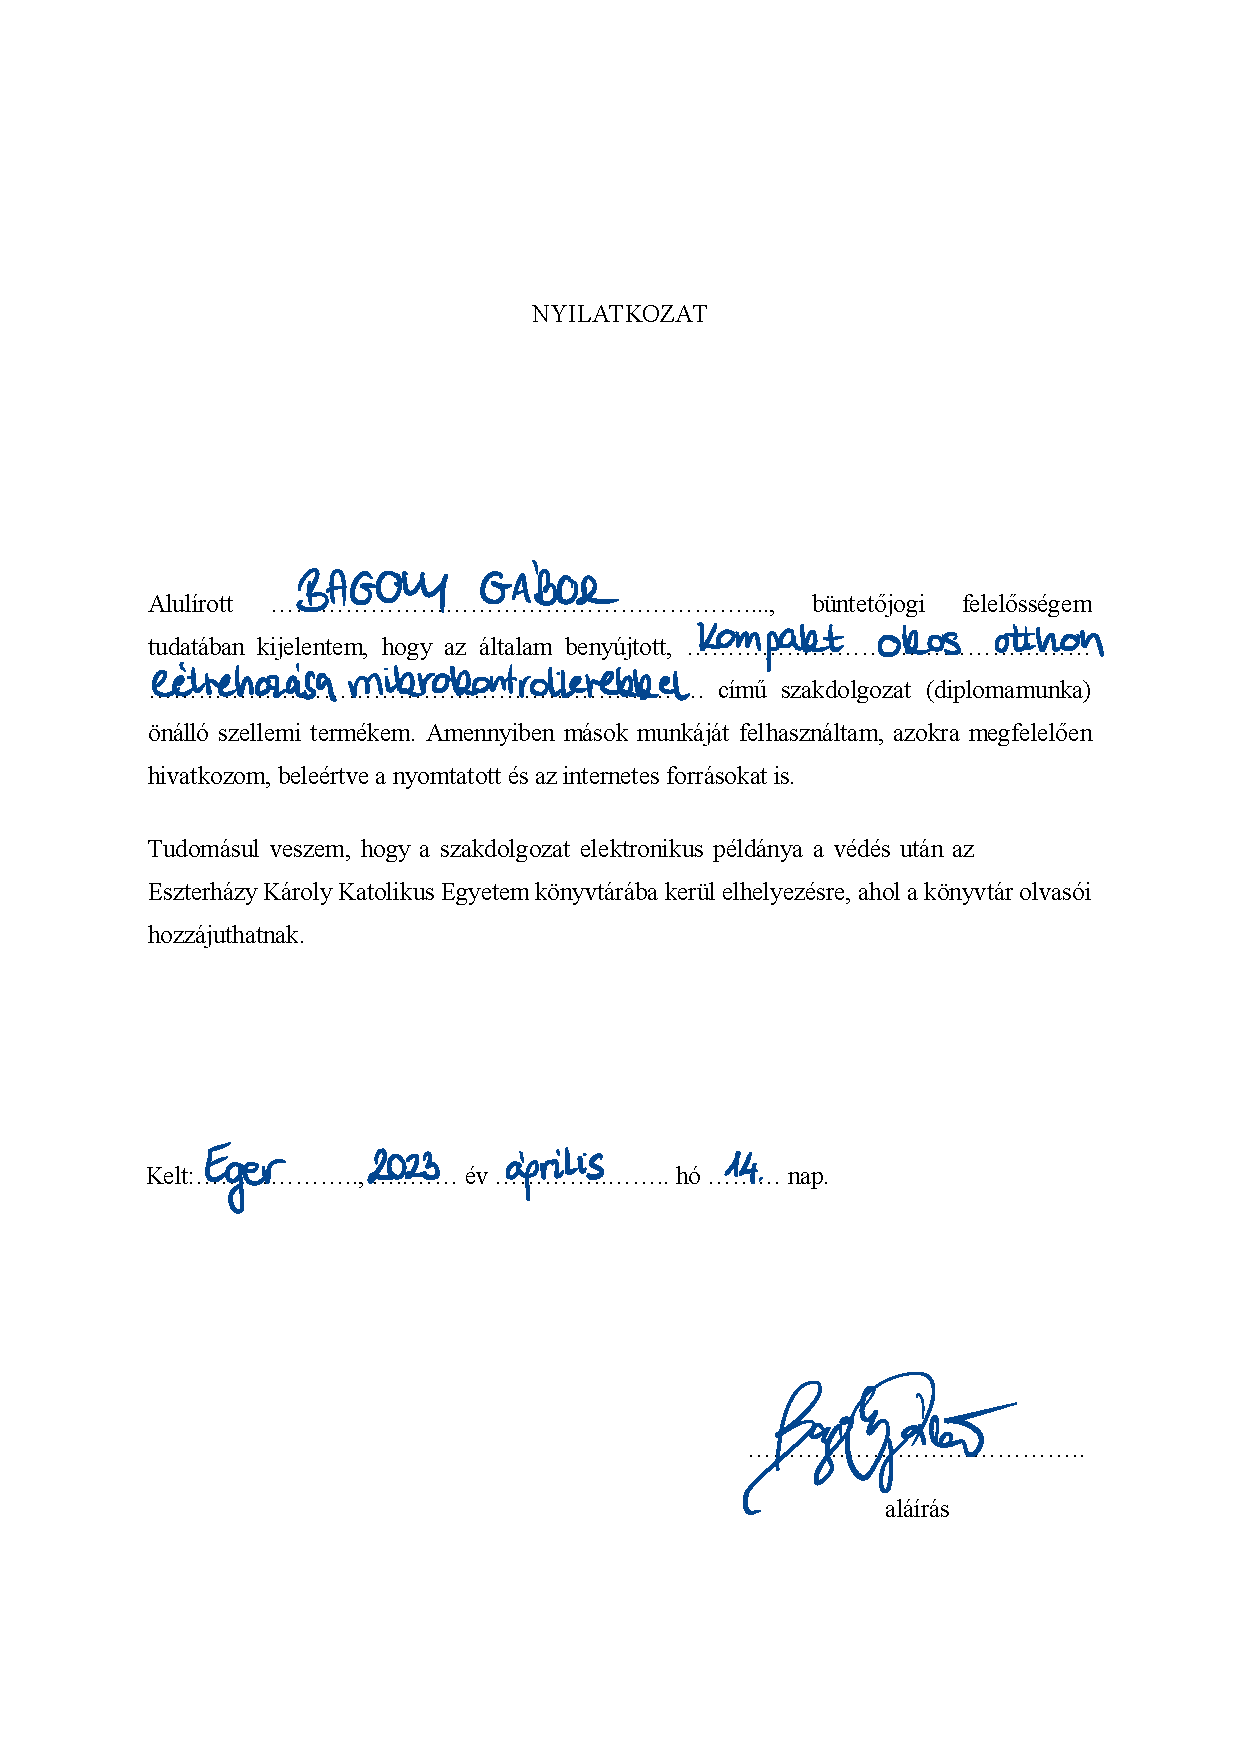
\includepdf{nyilatkozat.pdf}
\end{document}